\documentclass[../Dissertation.tex]{subfiles}

\begin{document}


%\emph{\color{red}
%\begin{itemize}
%	\item Questions to be addressed%
%	\item Metrics to be measured - why
%\end{itemize}
%}

This Chapter will discuss the methodology used to automate the search for lower latency models by tweaking pruning parameters.
Section~\ref{sec:EngineeringImplementation} explains how the pipeline was implemented, the discrete parts and how they all fit together.
Section~\ref{sec:ExperimentDesign} discusses the specifics of how we tested the system, the network model used and pruning algorithms selected.

\begin{figure}[H]
    \centering
    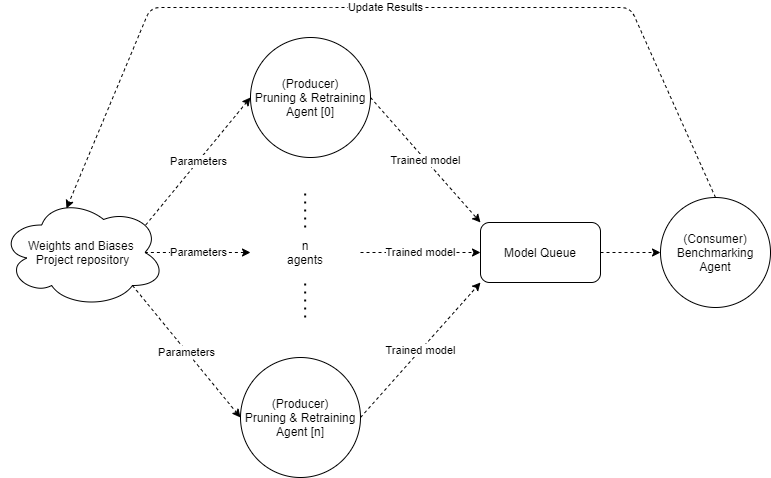
\includegraphics[width=1\textwidth]{./ProducerConsumer}
    \caption{Diagram showing communication between discrete parts of the system.}
    \label{fig:agentCommunication}
\end{figure}

%! ---------------------------------------------------------------------------------------------------------------------------------
\section{Automated pruning pipeline}\label{sec:EngineeringImplementation}

We constructed a pipeline to prune, retrain, benchmark, and record the data from each model, this pipeline consists of 4 separate elements; the systems to prune and retrain, a message queue  (for this we used Redis), a benchmarking system, and finally the cloud service used to store the data.
Figure~\ref{fig:agentCommunication} shows how each system interacts in the pipeline, pruning is handled by the agent/s marked `Producer', benchmarking is handled by the `Consumer' agent, and the \acrfull{wandb} system stores and provides the data used to compute each set of sweep parameters passed to the `Producer' agents on request.



When pruning begins, the producer agent uses initially random pruning parameters, the producer then applies the pruning algorithm, and begins retraining the model.
Upon completion of retraining the model is exported into ONNX format and added to a queue for the consumer (the benchmarking agent) to benchmark and record the results, these results are then logged to \acrshort{wandb}.
The parameter importance and correlation with the target metric is re-computed on each iteration of the pipeline using results that are logged to \acrshort{wandb} each time a benchmark is performed.

The runtime of a benchmark for a single model on the NCS is usually at most 5 seconds, retraining the network however can take between 20 - 120 mins depending on the network size and number of epochs, the one-shot pruning method utilised in this experiment usually takes less than 5 seconds. 
Because the training process is so slow we separated the benchmarking system (consumer) from the pruning and retraining systems (producer), this made it easy to add additional pruning and retraining agents to a single experiment or run multiple experiments in parallel.
To make use of this pipeline 2 files must be provided by the user, a distiller schedule with a definition for which weights will be pruned, and a \acrshort{wandb} configuration file which defines the type and ranges of the parameters it will seek to optimise.

%! ---------------------------------------------------------------------------------------------------------------------------------
\subsection{Defining parameters to prune}\label{sec:paramDef}

\singlespacing
\begin{figure}[H]
    \begin{minted}[breaklines, linenos]{yaml}
        pruners: 
            layer_1_conv_pruner:
                class: 'L1RankedStructureParameterPruner'
                group_type: Filters
                desired_sparsity: 0.9
                weights: [
                    module.layer1.0.conv1.weight,
                    module.layer1.1.conv1.weight
                ]
        lr_schedulers:
            exp_finetuning_lr:
                class: ExponentialLR
            gamma: 0.95

        policies:
            - pruner:
                instance_name: layer_1_conv_pruner
                epochs: [0]
            
            - lr_scheduler:
                    instance_name: exp_finetuning_lr
                starting_epoch: 10
                ending_epoch: 300
                frequency: 1
    \end{minted}
    \caption{Example distiller schedule file, showing the pruning algorithm selected, and that algorithms parameters}
    \label{fig:CompressionSchedule}
\end{figure}
\doublespacing

Distiller uses a `compression schedule' file to define the behaviour of the compression algorithms used, Figure~\ref{fig:CompressionSchedule} shows a simple example compression schedule, with a definition for a single `pruner' instance (line 2 - `'\texttt{\color{mintedgreen}layer\_1\_conv\_pruner}'), a single `\texttt{\color{mintedgreen}lr\_scheduler}' instance (line 11 - `\texttt{\color{mintedgreen}exp\_fine\_tuning\_lr}'), and their respective policies (explained below).


The pruning schedule is composed of lists of sections that describe `{\color{mintedgreen}pruners}', `{\color{mintedgreen}lr-schedulers}', and `{\color{mintedgreen}policies}'. 
A `{\color{mintedgreen}pruner}' defines a pruning algorithm and the layers on which that pruning algorithm will be applied, `LR-schedulers' define the \textbf{learning-rate decay(\color{red}Definition required)} algorithm. 
Finally each policy references an instance of a pruner or LR-scheduler, and controls when the respective algorithm will be applied, such as the start and end epoch, and the frequency of application.

The example compression schedule shown in Figure~\ref{fig:CompressionSchedule} provides instructions to Distiller to use the `L1RankedStructureParameterPruner' algorithm (as described in Section~\ref{sec:FilterPruningAlgo}) to prune the weights in each of the convolutions described by the `weights' array, in this case `\texttt{\color{mintedgreen}group\_type}' specifies filter pruning and `\texttt{\color{mintedgreen}desired\_sparsity}' indicates how many tensors it will aim to remove (0.9 indicates the algorithm will attempt to remove 90\% of the tensors), desired sparsity should not be confused with an actual change in sparsity | note that filter and channel pruning will always result in a dense layer with an actual sparsity of 0 because this is a form of coarse-grained pruning (see section~\ref{sec:Pruning}).

\begin{figure}[H]
    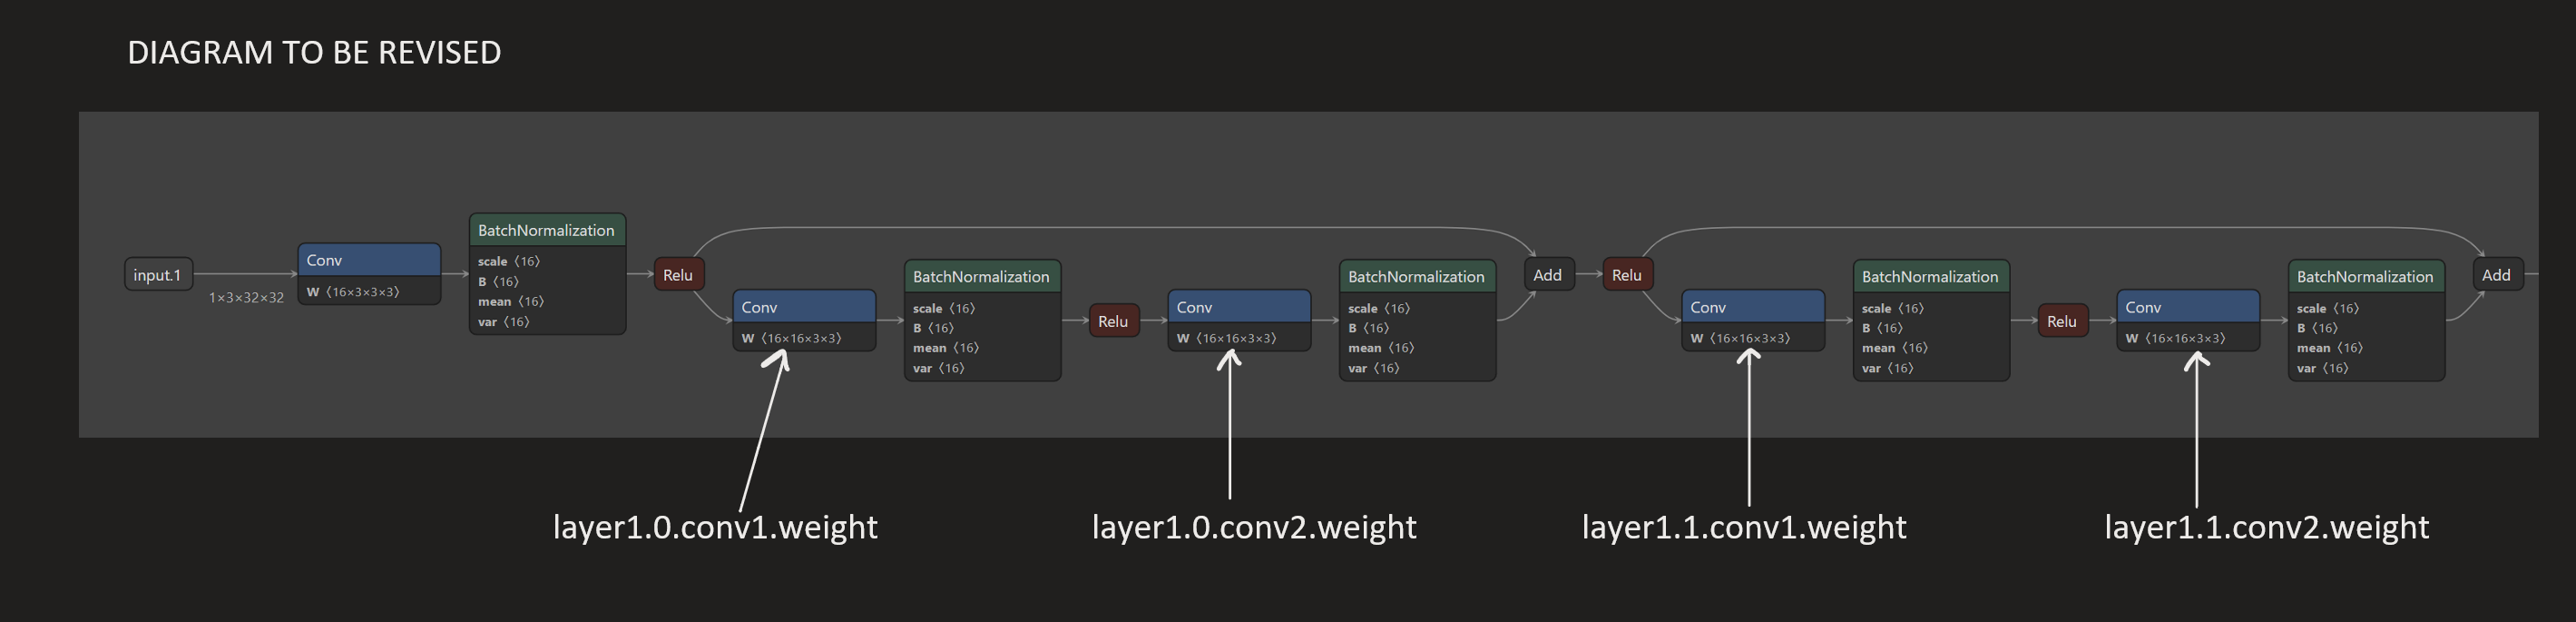
\includegraphics[width=\textwidth]{temp_pruning_layers.png}
    \caption{Resnet56 fragment showing first 2 residual block with the corresponding weights matrices labelled. \textbf{(TODO: rescale and redraw to highlight pertinent information)}}
    \label{fig:resnet56weightlabels}
\end{figure}

Each grouping of weights in the network has labels (see figure~\ref{fig:resnet56weightlabels}), distiller uses these labels to identify which weight matrices are being referenced by the compression schedule. 
Lines 7 and 8 in the schedule in Figure~\ref{fig:CompressionSchedule} reference the weights we wish to prune from the model in Figure~\ref{fig:resnet56weightlabels}.


\newpage
%! ---------------------------------------------------------------------------------------------------------------------------------
\subsection{WandB API}

\singlespacing
\begin{figure}[H]
    \begin{minted}[breaklines]{yaml}
        program: pipeline.py
        method: bayes
        metric:
            goal: minimize
            name: Latency
        parameters:
            layer_1_conv_pruner_desired_sparsity:
                min: 0.01
                max: 0.99
            layer_1_conv_pruner_group_type:
                values: [Channels, Filters]
    \end{minted}
    \caption{WandB sweep configuration file}
    \label{fig:sweepConfig}
\end{figure}
\doublespacing

To explore the space of pruning parameter values the hyperparameter optimisation framework exposed by WandB called `Sweeps' was leveraged. 
This involves writing a python script that can run the entire pipeline (pruning, training \& benchmarking) and record the results, to accomplish this each sweep needs a configuration file (see Figure~\ref{fig:sweepConfig}), table~\ref{tab:WandBConfig} shows a description of each key in the wandb configuration file with a summary of appropriate arguments. 


% which needs a definition to the python script being run (program), the search strategy (method, either grid, random, or bayes), a metric  

\begin{table}[H]
    \begin{tabular}{@{}|l|l|l|@{}}
    \toprule
    Key        & Description                    & Value                                    \\ \midrule
    program    & Script to be run               & Path to script                           \\ \midrule
    method     & Search strategy                & grid, random, or bayse                   \\ \midrule
    metric     & The metric to optimise         & Name and direction of metric to optimise \\ \midrule
    parameters & The parameter bounds to search & Name and min/max or array of fixed values  \\ \bottomrule
    \end{tabular}
    \caption{Configuration setting keys, descriptions and values}
    \label{tab:WandBConfig}
\end{table}


%E


The sweep configuration file tells wandb the names of the parameters to pass as arguments to the pipeline script with their expected value ranges, such as a list of strings or a min and max number. 
The pipeline script that receives the arguments from wandb contains a mapping from the wandb arguments to a corresponding value in a distiller compression schedule.
This is accomplished by parsing a base schedule file and identifying which values will be changed, then a new schedule is written with the parameters from wandb, this new schedule is then provided to Distiller as the compression schedule to use.



%! ---------------------------------------------------------------------------------------------------------------------------------
\subsection{Benchmarking}

\begin{figure}[H]
	\centering
	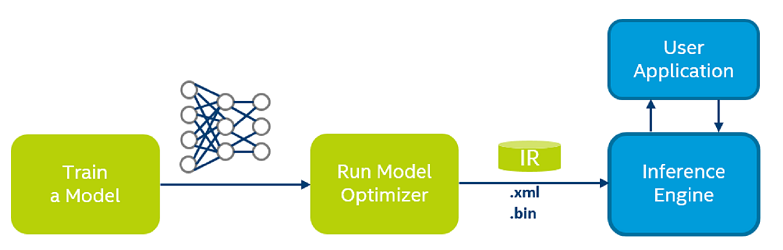
\includegraphics{./OpenVinoModelOptimizer}
	\caption{Workflow for deploying trained model onto NCS~\autocite{ModelOptimizerDeveloper}}
	\label{fig:OpenVinoWorkflow}
\end{figure}


To pass the pruned and trained model to the Neural Compute stick OpenVino was used, it is a toolkit providing a high level \textbf{inference engine(\color{red}Definition needed)} API, this facilitates the process of optimising the model for specialised hardware (in this case the NCS), and loading the optimised model into the hardware. 
OpenVino itself has a benchmarking tool that we leveraged to access detailed latency and throughput metrics; from end to end latency all the way down to the latency of each instruction used for inference on the VPU~\textbf{\color{red}link to example table of HW operations and latency in appendix}. 
Before starting the benchmark we convert the ONNX model into an Intermediate Representation (IR) format by running it through the model optimiser, the IR is then read by the Inference Engine and loaded into VPU memory.
Once the model is ready we load the images that will be used for benchmarking into the VPU memory.
We observe three measurements for every model, the end-to-end latency (from loading an image into the model until getting a result), the sum of latency for each instruction executed by the VPU once the image is loaded into memory, and finally we also measure the throughput (the number of images (frames) that can be processed per second or FPS).

%! ---------------------------------------------------------------------------------------------------------------------------------
\newpage

%! ---------------------------------------------------------------------------------------------------------------------------------
\section{Experiment Design}\label{sec:ExperimentDesign}

\subsection{Filter Pruning algorithm}\label{sec:FilterPruningAlgo}
We selected the one-shot pruning algorithm dubbed `L1RankedStructureParameterPruner' by Distiller, this is based on the algorithm described by Li et al. in Pruning Filters for Efficient Convnets~\autocite{liPruningFiltersEfficient2017}. 
We prune the filters that are expected to have the smallest impact on the accuracy of the network, this is determined by computing the sum of the absolute weights in each filter $\Sigma~|\mathcal{F}_{i,j}|$, sorting them, and pruning the filters starting with the smallest sum values.
Each filter that gets removed causes the corresponding feature map to be removed, along with its corresponding kernel in the next convolutional layer, see Figure~\ref{fig:FeaturemapAndKernel}. \\


\begin{singlespace}
\noindent Li et al~\autocite{liPruningFiltersEfficient2017} defines the procedure for pruning $m$ filters from the $i$th convolutional layer as follows:

\noindent Let $n_i$ denote the number of input channels.
    \begin{enumerate}
        \item For each filter $\mathcal{F}_{i,j}$, calculate the sum of its absolute kernel weights $s_{j} = \Sigma_{l=1}^{n_{i}}\Sigma~|\mathcal{K}_{l}|$.
        \item Sort the filters by $s_j$.
        \item Prune $m$ filters with the smallest sum values and their corresponding feature maps. The kernels in the next convolutional layer corresponding to the pruned feature maps are also removed.
        \item A new kernel matrix is created for both the $i$th and $i + 1$th layers, and the remaining kernel weights are copied to the new model.
    \end{enumerate}
\end{singlespace}

\noindent Upon completion of pruning the filters we now retrain the network to regain lost accuracy, in general pruning the more resilient layers once and retraining can result in much of the lost accuracy to be regained.
Once pruning is completed we compensate for the performance degradation by retraining the network, 

    \begin{figure}[H]
        \centering
        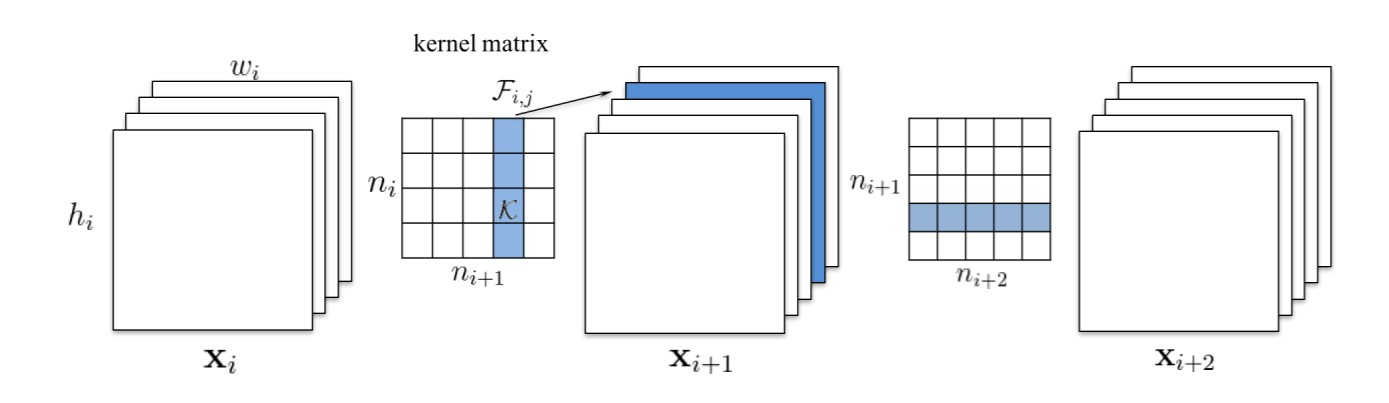
\includegraphics[width=0.8\textwidth]{FilterPruning.jpg}
        \caption{Pruning a filter results in removal of its corresponding feature map and related kernels in the next layer.~\autocite{liPruningFiltersEfficient2017}\textbf{\color{red}Include annotations for the feature map and kernel}}
        \label{fig:FeaturemapAndKernel}
    \end{figure}




%! ---------------------------------------------------------------------------------------------------------------------------------
\subsection{Model Selection}\label{sec:ModelSelection}

Pruning CNNs like AlexNet, or VGGNet is fairly straightforward, we can prune filters in any layer without worrying about damaging the fundamental structure of the network, however this is not the case with ResNets (short for Residual Networks),  a very popular type of CNN that makes use of what is known as a `residual block' (Figure~\ref{fig:ResidualBlock} shows a residual block) which, from the perspective of pruning, adds additional interdependencies between layers.

We selected ResNet56 as the target network because it is one of the few networks with prebuilt `off-the-shelf' schedules that also uses residual blocks. 
Performing this experiment on networks using residual blocks is important because the necessity of using compression techniques such as pruning increases as networks get larger, these residual blocks are very common in very large networks today. 

The pre-tuned pruning schedule publicly available from Distiller has been hand built by an expert in the field, providing a solid baseline for comparison.
It is not a trivial task to improve on the pre-existing hand built schedules manually without extensive understanding of layer sensitivities.  

\begin{figure}[H]
    \centering
    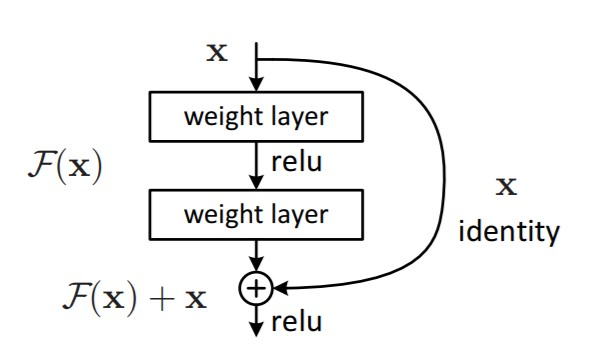
\includegraphics[width=0.5\textwidth]{ResidualBlock.jpg}
    \caption{A residual block, note the identity feature map skips the weight layers, this is also known as a `skip connection'.}
    \label{fig:ResidualBlock}
\end{figure}

\textbf{\color{red}Discuss further how residual blocks effect pruning.}
ResNets were originally proposed to help address a training accuracy degradation problem that can occur in very deep networks, degradation (or accuracy saturation) occurs when adding more layers to a suitably deep model leads to higher training error~\autocite{heDeepResidualLearning2016}.
The accuracy degradation problem with very deep CNNs is common enough that many new deep networks in research and production make use of them today.

%! ---------------------------------------------------------------------------------------------------------------------------------
\subsection{Optimisation Process}
In general machine learning algorithms are expensive to perform, and tend to have an inconsistent execution time, when the cost of retraining is so high it is easy to see why we would want to exchange some extra work up front for finding a good next search point rather than simply relying on the more commonly used hill climbing algorithms that rely more on the local gradient.
One of the key ideas here is to use all information available from all previous function evaluations, allowing us to model the plausibility of future search points, Bayesian optimisation processes are designed to construct this model by evaluating this prior knowledge about known properties, these are considered to be some of the most effective optimisation approaches in terms of the number of function evaluations required~\autocite{brochuTutorialBayesianOptimization2010}.

The specific flavour of Bayesian optimisation process used in this dissertation is based on the method described by Snoek et al.~\autocite{snoekPracticalBayesianOptimization2012} where statistical models are used to find search points heuristically using a Monte Carlo estimate of the expected improvement.
 
Due to the stochastic nature of the pruning methods we have utilised there is a considerable volume of noise in our data because when we perform optimisation we tune all pruners in parallel, each pruner will have a different degree of impact on the target metric

%! ---------------------------------------------------------------------------------------------------------------------------------
\subsection{Experiment metrics and parameters}\label{sec:metricsandparams}


We conducted three experiments using a Resnet56 model with pretrained weights for the CIFAR10 dataset.
This section describes the parameters and metrics that will be either set or observed during the experiments.

\singlespacing
\noindent\textbf{Parameters:}
\begin{itemize}
    \item \textbf{Desired Sparsity} | Specified on a per-pruner basis, this lets us specify to the pruning algorithm what proportion of the weights to try and prune (See Section~\ref{sec:paramDef} for more details).
    \item \textbf{Epochs} | The number of epochs used for retraining, one epoch refers to a single cycle of training through the entire training dataset.
    \item \textbf{Learning Rate} | Used to scale how much the retraining process will adjust the weights during each weight update.
    \item \textbf{Group type} | Specify either `Filters' or `Channels' for pruning. \textbf{\color{red}Extend background with stuff about channels/filters}.
\end{itemize}
\doublespacing

\singlespacing
\noindent\textbf{Observed metrics:}
\begin{itemize}
    \item \textbf{Latency} | Computed by calculating the sum of CPU time for hardware operations inside the NCS after the model and images have been loaded into memory.
    \item \textbf{Total\_Latency} | Measures the full latency to perform inference on an image once a model is optimised and loaded into the NCS, including loading the image into the stick memory, this is more indicative of real world requirements.
    \item \textbf{Throughput} | Shows the number of images per second that can be processed by the NCS (Frames Per Second).
    \item \textbf{Top1} | The \% accuracy of the first class predicted by the model.
    \item \textbf{Top5} | The \% accuracy of the first 5 classes the model predicted for a given image.
\end{itemize}
\doublespacing

\newpage
\subsection{Schedules}
Table~\ref{tab:scheduleWeights} shows how the weights are grouped and labeled for pruning in the selected Resnet56 model, the 4 labelled pruners and their corresponding weights were used in all resnet56 experiments.
Layers with a similar degree of sensitivity to pruning are grouped together, layers that are omitted from the table have a much higher sensitivity to pruning and are not pruned at all, pruning more sensitive layers can result in a significantly higher probability that pruned neural networks that lose all predictive ability (in other words the network will predict a single class 100\% of the time).
Grouping layers in this way helps us avoid having to use 56 pruning parameters (one for each layer per residual block) and significantly reduces the complexity of the parameter search.
Note that only the first convolution in each residual block is being pruned (denoted by `conv1' inside the weight name), because the convolutions following this will also have the kernels removed following the removed feature maps (See Section~\ref{sec:ModelSelection}).

\singlespacing
\begin{table}[H]
    \centering
    \setlist[itemize]{font= \color{black}, wide, leftmargin=*, noitemsep, after=\vspace*{-\topsep}}
    \setlength{\extrarowheight}{0.5pt}
    \setlength{\tabcolsep}{3pt}
    \begin{tabularx}{0.6\textwidth}{|p{40mm}|*{1}{>{\compress\RaggedRight\arraybackslash} X |}}
    \hline
    Label & Weights  \\
    \hline
    filter\_pruner\_layer\_1
    & \begin{itemize}
        \item module.layer1.0.conv1.weight
        \item module.layer1.1.conv1.weight
        \item module.layer1.2.conv1.weight
        \item module.layer1.3.conv1.weight
        \item module.layer1.4.conv1.weight
        \item module.layer1.5.conv1.weight
        \item module.layer1.6.conv1.weight
        \item module.layer1.7.conv1.weight
        \item module.layer1.8.conv1.weight
    \end{itemize} \\ 
    \hline
    filter\_pruner\_layer\_2 
    & \begin{itemize}
        \item module.layer2.1.conv1.weight
        \item module.layer2.2.conv1.weight
        \item module.layer2.3.conv1.weight
        \item module.layer2.4.conv1.weight
        \item module.layer2.6.conv1.weight
        \item module.layer2.7.conv1.weight
    \end{itemize} \\ 
    \hline
    filter\_pruner\_layer\_3.1
    & \begin{itemize}
        \item module.layer3.1.conv1.weight
    \end{itemize} \\
    \hline
    filter\_pruner\_layer\_3.2
    & \begin{itemize}
        \item module.layer3.2.conv1.weight
        \item module.layer3.3.conv1.weight
        \item module.layer3.5.conv1.weight
        \item module.layer3.6.conv1.weight
        \item module.layer3.7.conv1.weight
        \item module.layer3.8.conv1.weight
    \end{itemize}\\ \hline
    \end{tabularx}
    \caption{Mapping of pruners labels to resnet56 weights}
    \label{tab:scheduleWeights}
\end{table}
\doublespacing

\subsection{Passing pruned/trained networks to benchmark}
\emph{\color{red}Discuss reading/writing yaml files, outputting .onnx files, redis to pass messages between agents}

\subsection{Baseline data}\label{sec:baselineData}
For the purposes of all experiments we compare our results to two baseline sets of data, first the basic ResNets56 network with pretrained weights for CIFAR10 no pruning, and second an `off-the-shelf' version of ResNet56 with pruning parameters hand-picked by the researcher responsible for development of Distiller (thus it is highly likely to be used as a starting point for new users to distiller)~\autocite{liPruningFiltersEfficient2017}.

\begin{table}[H]
    \begin{tabular}{@{}lccp{25mm}p{23mm}p{28mm}@{}}
    \toprule
    \multicolumn{1}{c}{\textbf{Model}} & \textbf{Top1} & \textbf{Top5} & \textbf{Throughput (FPS)} & \textbf{Latency (ms)} & \textbf{Total Latency (ms)} \\ \midrule
    Baseline - no pruning              & 92.58         & 99.78         & 294.08                    & 4.375                 & 13.19                       \\
    Off the shelf - no retraining      & 11.19         & 51.02         & 303.98                    & 3.947                 & 12.89                       \\
    Off the shelf - retrained          &  87.72        & 99.47         & 305.27                    & 3.88                  & 12.95                           \\ \bottomrule
    \end{tabular}
\end{table}

\subsection{Experiment 1: Rapid pruning, no retraining}~\label{sec:ex1}
Targeting the weights described in table~\ref{tab:scheduleWeights} (the full schedule is listed in appendix~\ref{apx:Schedule}) we repeatedly pruned networks without performing any training to regain accuracy, we set the target metric to minimize Latency, the number of epochs to $0$, and the learning rate to $0.1$.
The goal at this stage was to observe any reduction in latency, with the added benefit of allowing us to gather a large volume of data very quickly.
Figure~\ref{fig:LatencySweepConfig} shows the wandb configuration file used for this degradation, this configuration seeks to optimise the desired sparsity settings for each of the 4 pruners.

\singlespacing
\begin{figure}[H]
    \centering
    \begin{minted}[breaklines]{yaml}
program: pipeline.py
method: bayes
metric:
  goal: minimize
  name: Latency
parameters:
  filter_pruner_layer_1:
    min: 0.0
    max: 0.99
  filter_pruner_layer_2:
    min: 0.0
    max: 0.99
  filter_pruner_layer_3.1:
    min: 0.0
    max: 0.99
  filter_pruner_layer_3.2:
    min: 0.0
    max: 0.99
    \end{minted}
    \caption{Targeting Latency sweep config}
    \label{fig:LatencySweepConfig}
\end{figure}
\doublespacing

\subsection{Experiment 2: Target latency, with retraining}

Using the same wandb configuration file as in the first experiment (Figure~\ref{fig:LatencySweepConfig}), we again target minimizing latency but this time retrain for a fixed $70$ epochs, and set the learning rate to $0.1$.
The purpose of this part of the experiment was to observe how well the optimisation process targeting only latency could recover accuracy.

\subsection{Experiment 3: Target Top1, with retraining}
During the third experimental stage we tweaked the configuration file (see Figure~\ref{fig:Top1SweepConfig}) to specify a new target metric: maximise Top1 .
Similarly to Experiment 2 we kept the number of epochs fixed at $70$ and the learning rate at $0.1$.
During this experiment we were interested in observing how the amount of pruning effected Top1, and if we could improve on our best Top1 score from the second experiment.

\singlespacing
\begin{figure}[H]
    \centering
    \begin{minted}[breaklines]{yaml}
program: pipeline.py
method: bayes
metric:
  goal: maximize
  name: Top1
parameters:
  filter_pruner_layer_1:
    min: 0.0
    max: 0.99
  filter_pruner_layer_2:
    min: 0.0
    max: 0.99
  filter_pruner_layer_3.1:
    min: 0.0
    max: 0.99
  filter_pruner_layer_3.2:
    min: 0.0
    max: 0.99
    \end{minted}
    \caption{Targeting Latency sweep config}
    \label{fig:Top1SweepConfig}
\end{figure}
\doublespacing

\subsection{Experiment 4: Adding epochs and learning rate to the parameter search}




\end{document}